
%importa variabili utili
%%Variabili globali
\def\GRUPPO			{\textbf{$M^5$}}
\def\INDIRIZZO		{indirizzo}

\def\PROGETTO		{Sviluppo di un sistema informatico per la gestione dei contenuti non strutturati presenti in newsletter inviate via e-mail}
\def\SIGLA			{ECM-1.0}

\def\NOMEPROGETTO	{\textit{MailForYou}}
\def\SIGLAPROGETTO	{\textit{M4U}}

\def\COMMITTENTE	{Prof. Ghiraldo Filippo}

\def\EMAIL			{malla5.sgp@gmail.com}


\def\LOGO			{../template/img/loghi/logoM4Y.png}
\def\INTESTAZIONE	{../template/img/loghi/intestazione.png}
\def\PIEDIPAGINA	{../template/img/loghi/piedipagina.png}

%Scorciatoie
\def\fasi#1{\textbf{#1}\xspace}
\def\rev#1{\textbf{#1}\xspace}
\def\role#1{\textit{#1}\xspace}
\def\doc#1{\textit{#1}\xspace}
\def\code#1{\hl{\texttt{#1}}\xspace}
\def\path#1{\texttt{#1}\xspace}
\def\glo#1{#1$_{_{G}}$\xspace}
\def\ignoreglo#1{#1\xspace}


\def\INDICE		{true} 		%abilita - disabilita l'indice
\def\TABELLE	{true} 		%abilita - disabilita l'indice delle tabelle
\def\FIGURE		{true} 		%abilita - disabilita l'indice delle figure

%importa la struttura
% aggiunto riga sotto per risolvere problema di visualizzazione su Acrobat Reader sun W7
% http://tex.stackexchange.com/questions/64448/how-to-overcome-acrobat-reader-error-131-with-a-pdflatex-doc
\pdfminorversion=4
\documentclass[a4paper,11pt]{article}

%Non modificare
%*****nuovi comandi************************
%fornisce il caption per riferirsi ad una particolare sezione
\newcommand{\numref}[1]{\textsf{\textsl{``\nameref{#1}'' (\ref{#1})}}}
%**IMPORTAZIONE PACKAGE**************************
\usepackage{ifthen}
\usepackage[T1]{fontenc}
\usepackage[utf8]{inputenc}
\usepackage[italian]{babel}
\usepackage{xspace}
\usepackage{float}
\usepackage{chapterbib}
\usepackage{graphicx, subfigure}
\usepackage[a4paper,top=3cm,bottom=3cm,left=3cm,right=3cm,bindingoffset=5mm]{geometry}
\usepackage[colorlinks=true, urlcolor=blue, citecolor=black, linkcolor=black, hyperindex, breaklinks]{hyperref}
\usepackage{booktabs}
\usepackage{totpages}
\usepackage{tabularx, array}
\usepackage{dcolumn}
\usepackage{epstopdf}
\usepackage{booktabs}
\usepackage{fancyhdr}
\usepackage{longtable}
\usepackage{multirow}
\usepackage{calc}
\usepackage{eurosym}
\usepackage{datatool}
\usepackage[bottom]{footmisc}
\usepackage{listings} % used to report code
\usepackage{verbatim}
\usepackage{enumitem}
\usepackage{titlesec}
\usepackage[nonumberlist,acronym,toc]{glossaries}
\usepackage{tikz}
\usepackage{amssymb}
\usepackage{wallpaper}
\usepackage{grffile}
\usepackage{soul}
%\usepackage{floatflt}
\usepackage{pgf}
\usepackage{caption}
\usepackage{subfigure}
\hypersetup{colorlinks=true, linkcolor=blue, anchorcolor=blue, urlcolor=blue} 

\captionsetup{tableposition=top, figureposition=bottom, font=small}


%scalegraphics
\makeatletter
\def\ScaleIfNeeded{%
\ifdim\Gin@nat@width>\textwidth
  \textwidth
\else
  200px
\fi
}
\makeatother
\def\scalegraphics#1{
  \includegraphics[width=\ScaleIfNeeded]{#1}
}

%glossary
\newglossarystyle{altlistgroupmod}{
\glossarystyle{altlistgroup}
\renewcommand{\glsgroupskip}{} 
}
\glossarystyle{altlistgroupmod}

% Listings
\usepackage{listings}
\usepackage{color}

\definecolor{dkgreen}{rgb}{0,0.6,0}
\definecolor{dkred}{rgb}{0.6,0,0}
\definecolor{gray}{rgb}{0.5,0.5,0.5}
\definecolor{mauve}{rgb}{0.58,0,0.82}
\definecolor{light-gray}{gray}{0.95}

\lstset{
  language=C++,
  aboveskip=3mm,
  belowskip=3mm,
  showstringspaces=false,
  columns=flexible,
  basicstyle={\small\ttfamily},
  numbers=none,
  numberstyle=\tiny\color{gray},
  keywordstyle=\color{blue},
  commentstyle=\color{dkgreen},
  stringstyle=\color{mauve},
  breaklines=true,
  breakatwhitespace=true
  tabsize=3
}

%soul color
\sethlcolor{light-gray}

%Tikz tree
\makeatletter
\newcount\dirtree@lvl
\newcount\dirtree@plvl
\newcount\dirtree@clvl
\def\dirtree@growth{%
  \ifnum\tikznumberofcurrentchild=1\relax
  \global\advance\dirtree@plvl by 1
  \expandafter\xdef\csname dirtree@p@\the\dirtree@plvl\endcsname{\the\dirtree@lvl}
  \fi
  \global\advance\dirtree@lvl by 1\relax
  \dirtree@clvl=\dirtree@lvl
  \advance\dirtree@clvl by -\csname dirtree@p@\the\dirtree@plvl\endcsname
  \pgf@xa=1cm\relax
  \pgf@ya=-0.5cm\relax
  \pgf@ya=\dirtree@clvl\pgf@ya
  \pgftransformshift{\pgfqpoint{\the\pgf@xa}{\the\pgf@ya}}%
  \ifnum\tikznumberofcurrentchild=\tikznumberofchildren
  \global\advance\dirtree@plvl by -1
  \fi
}

\tikzset{
  dirtree/.style={
    growth function=\dirtree@growth,
    every node/.style={anchor=north},
    every child node/.style={anchor=west},
    edge from parent path={(\tikzparentnode\tikzparentanchor) |- (\tikzchildnode\tikzchildanchor)}
  }
}
\makeatother

% Glossaries
\makeglossaries
\renewcommand*{\glspostdescription}{}
\renewcommand*{\glssymbolsgroupname}{Simboli}%


% Aumento profondità subsections
\setcounter{secnumdepth}{4}

\titleformat{\paragraph}
{\normalfont\normalsize\bfseries}{\theparagraph}{1em}{}
\titlespacing*{\paragraph}
{0pt}{3.25ex plus 1ex minus .2ex}{1.5ex plus .2ex}

%**STILE PAGINA**********************************
\renewcommand{\subsectionmark}[1]{%
  \ifsubsectioninheader
    \def\subsectiontitle{: #1}%
  \else
    \def\subsectiontitle{}%
  \fi
}  

\fancypagestyle{stilecapitolinumerati}{
\pagestyle{fancy}
\fancyhf{}
\newif\ifsubsectioninheader
\def\subsectiontitle{}


\fancyhead[L]{\nouppercase{\rightmark\ifsubsectioninheader\subsectiontitle\fi}}

%LE,RO
\fancyhead[R]{\nouppercase{\slshape\leftmark}}
\rfoot{\thepage ~di~\pageref{TotPages}}
\renewcommand{\headrulewidth}{1.5pt}
\renewcommand{\footrulewidth}{1.5pt}
}

\fancypagestyle{stilecapitolinonnumerati}{
\pagestyle{fancy}
\fancyhf{}
\rfoot{\thepage ~di~\pageref{TotPages}}
\renewcommand{\headrulewidth}{1.5pt}
\renewcommand{\footrulewidth}{1.5pt}
}

%no indentazione paragrafo
\setlength{\parindent}{0pt}

\setlength{\headheight}{25pt}

%**PRIMA PAGINA***************************

\begin{document}
%Centra il testo
%**************************************************************
% file contenente le impostazioni della tesi
%**************************************************************

%**************************************************************
% Frontespizio
%**************************************************************
\newcommand{\myName}{Marco Baesso}                                    % autore
\newcommand{\myTitle}{Manutenzione adattativa di un software opensource}                    
\newcommand{\myDegree}{Tesi di laurea triennale}                % tipo di tesi
\newcommand{\myUni}{Università degli Studi di Padova}           % università
\newcommand{\myFaculty}{Corso di Laurea in Informatica}         % facoltà
\newcommand{\myDepartment}{Dipartimento di Matematica}          % dipartimento
\newcommand{\myProf}{Silvia Crafa}                                % relatore
\newcommand{\myLocation}{Padova}                                % dove
\newcommand{\myAA}{2012-2013}                                   % anno accademico
\newcommand{\myTime}{Ottobre 2013}                                  % quando


%**************************************************************
% Frontespizio 
%**************************************************************
\begin{titlepage}

\begin{center}

\begin{LARGE}
\textbf{\myUni}\\
\end{LARGE}

\vspace{10pt}

\begin{Large}
\textsc{\myDepartment}\\
\end{Large}

\vspace{10pt}

\begin{large}
\textsc{\myFaculty}\\
\end{large}

\vspace{30pt}
\begin{figure}[htbp]
\begin{center}

\includegraphics[height=6cm]{../template/img/logo-unipd}
\end{center}
\end{figure}
\vspace{30pt} 

\begin{LARGE}
\begin{center}
\textbf{\myTitle}\\
\end{center}
\end{LARGE}

\vspace{10pt} 

\begin{large}
\textsl{\myDegree}\\
\end{large}

\vspace{40pt} 

\begin{large}
\begin{flushleft}
\textit{Relatore}\\ 
\vspace{5pt} 
Prof. \myProf
\end{flushleft}

\vspace{0pt} 

\begin{flushright}
\textit{Laureando}\\ 
\vspace{5pt} 
\myName
\end{flushright}
\end{large}

\vspace{40pt}

\line(1, 0){338} \\
\begin{normalsize}
\textsc{Anno Accademico \myAA}
\end{normalsize}

\end{center}
\end{titlepage} 

\newpage

%si usa la numerazione romana per gli indici e la tabella delle modifiche
\pagenumbering{Roman}
%************************************************


\twocolumn
\newgeometry{top=8cm,bottom=5cm}
\section*{Sommario}
Questo documento intende presentare il lavoro svolto durante il mio stage all'interno dell'azienda RDS-NORDEST.\\ \\
Il lavoro � stato preceduto da una pianificazione delle attivit� identificando gli obiettivi di minimo e di massimo previsti per il progetto.\\ \\
Partendo dalla fase di analisi dei requisiti sono stati definiti i vincoli del progetto per poi continuare con la progettazione, la codifica e la verifica;\\ \\ ogni fase del progetto � stata documentata in modo da tenere aggiornato e visibile a tutti lo stato del software.\\ \\
Il documento rappresenta la relazione dello stage da me svolto fornendo quindi i dettagli tecnici minimi per la comprensione del progetto e dei problemi riscontrati.

\restoregeometry

\newpage

%importa gli indici
%************************************************
%Inserisce il link all'indice
%\addcontentsline{toc}{section}{Indice}
\ifthenelse{\equal{\INDICE}{true}} 
{\tableofcontents \newpage}

%se è stata impostata a true la variabile per la lista delle tabelle, la mostra
\ifthenelse{\equal{\TABELLE}{true}} 
{\listoftables \newpage}{}

%se è stata impostata a true la variabile per la lista delle figure, la mostra
\ifthenelse{\equal{\FIGURE}{true}}
{\listoffigures \newpage}{}

%da qui comincia la numerazione normale
\pagenumbering{arabic}

%separatore per individuare l'inizio del testo
\iffalse
AOjvdYTJD7mcIIYItfsNiYPbmTTogRSP9hrrb2XPE1laMyQ9NHrPgTCTxnW0eV1YcM3Wqh7t5qThjczeXWq3O5FJ7BBQjoWZovC5
\fi

\pagestyle{stilecapitolinumerati}

\section{Dominio applicativo}
\subsection{Azienda ospitante}
\input{sections/dominio/azienda}

\subsection{Descrizione dello stage}
La pianificazione iniziale prevedeva come obiettivo minimo la realizzazione di uno schedulatore di attivit\`{a} ad hoc per laboratori che effettuano analisi chimiche, fisiche e merceologiche per conto terzi. L\textquoteright{}obiettivo di massimo era l\textquoteright{}integrazione dello schedulatore con un software in fase di sviluppo da parte dell\textquoteright{}azienda. Il tutto doveva essere preceduto dalla scelta della tecnologia da utilizzare per la realizzazione dello schedulatore.
A inizio stage la scelta della tecnologia \`{e} stata convenuta dall\textquoteright{}azienda. La soluzione consisteva nella modifica di un software opensource la cui funzionalit\`{a} era proprio quella di realizzare la pianificazione dei progetti utilizzando come strumento tecnico di pianificazione il diagramma di Gantt. Il software opensource pu\`{o} essere scaricato dalla piattaforma di SourceForge al seguente indirizzo: \url{http://sourceforge.net/projects/opproject/}.
Il software purtroppo \`{e} privo di documentazione, gli unici documenti reperibili sono i sorgenti dell\textquoteright{}applicativo scritti utilizzando il linguaggio Java. L\textquoteright{}adozione di questa soluzione \`{e} stata preceduta da uno studio di fattibilit\`{a} da parte dell\textquoteright{}azienda stessa, che a mio parere ha posto pi\`{u} attenzione ai pro della soluzione piuttosto che agli aspetti a sfavore nella scelta intrapresa. Infatti l\textquoteright{}applicativo \`{e} gi\`{a} sviluppato, ma essendo privo di documentazione, la sua manutenzione, adattativa e correttiva, nel caso in questione rischier\`{a} di far perdere all\textquoteright{}azienda molto tempo soprattutto perch\`{e} non \`{e} stato richiesto di integrare la parte di documentazione mancante all\textquoteright{}applicativo, quindi se l\textquoteright{}azienda dovesse apportare delle modifiche dovr\`{a} procedere prima con delle fasi di debugging al fine di comprendere le dinamiche del software per poi poter applicare le modifiche, il risultato finale \`{e} una pessima efficienza. Le ragioni di ci\`{o} sono testimoniate dall\textquoteright{}esperienza da me acquisita durante il progetto, per dare un\textquoteright{}idea quantitativa il software consiste in pi\`{u} di 1000 classi.
L\textquoteright{}azienda adottando la soluzione scelta ha immediatamente cambiato le milestones del mio progetto di stage. L\textquoteright{}obiettivo da raggiungere era proprio la realizzazione dello schedulatore ad hoc. Consultare la sezione di \nameref{sec:analisi} per i dettagli su quello che deve essere lo schedulatore ad hoc. La pianificazione quindi vede in aggiunta una fase di debugging inizialmente non prevista, e visti i tempi previsti per la durata dello stage, circa 300 ore \`{e} stata convenuta la rimozione dell\textquoteright{}obiettivo di massimo, da prevedere in un momento successivo, ma non nella baseline del mio progetto.

\subsection{Pianificazione}
In questa sezione vengono riportati i diagrammi di Gantt che forniscono una visione a preventivo del progetto a me commissionato. Nel primo diagramma si ha la visione della pianificazione delle attivit\`{a} prima di intraprendere il progetto.

Questo \`{e} il diagramma che \`{e} stato modificato in relazione alla scelte implementative dell\textquoteright{}azienda.

Un diagramma di Gantt a preventivo, come quelli presentati, si dimostra utile per capire quali sono le dipendenze delle attivit\`{a}, la loro durata (meglio con un diagramma di Pert), le scadenze. I diagrammi di Gantt a consuntivo possono essere utilizzati come strumento di misurazione dell\textquoteright{}abilit\`{a} di un project Manager nella pianificazione dei progetti, tale strumenti quindi possono essere utilizzati al fine di mirare al miglioramento continuo in logica PDCA.

\paragraph{Ciclo di vita}
Il modello di ciclo di vita dell\textquoteright{}azienda rientra tra le metodologie agili. L\textquoteright{}azienda settimanalmente produce il cosidetto \textit{``sprint planning\textquoteright{}\textquoteright{}} ovvero pianifica le attivit\`{a} da svolgere nella settimana successiva. A questa fase si susseguono le attivit\`{a} di verifica pianificate, sia relative allo stato di avanzamento del prodotto sia relative alla qualit\`{a} del prodotto. In relazione al ciclo di vita adottato dall\textquoteright{}azienda ovviamente con gli stagisti ha adottato lo stesso approcio fornendo sul mio progetto revisioni eseguite con una frequenza pari a 2 settimane. Il progetto da me svolto per le caratteristiche presentate si \`{e} concordato con il modello dell\textquoteright{}azienda per quanto riguarda i processi di revisione e di comunicazione; tuttavia \`{e} stato indispensabile adottare per il progetto un ciclo di vita incrementale, nello specifico sono stati pianificati e poi mantenuti 3 incrementi. La natura del ciclo adottata \`{e} stata incrementale proprio a causa del modello adottato dall\textquoteright{}azienda. Infatti il dettaglio dei requisiti del progetto, sono emersi non dall\textquoteright{}inizio ma durante lo stage e quindi durante il ciclo di vita stesso. Il progetto quindi ha prodotto un software la cui vita \`{e} stata animata da baseline successive.
\newpage

\section{Analisi dei requisiti}
\label{sec:analisi}
Durante l\textquoteright{}attivit\`{a} di stage sono stati riassunti i requisiti specificati per il progetto in diagrammi dei casi d\textquoteright{}uso al fine di specificare nella maniera pi\`{u} chiara e semplice possibile le specifiche per il progetto. In questa sezione viene presentato il minimo indispensabile per far comprendere quello in cui consisteva il dominio del progetto.  

\subsection{Casi d\textquoteright{}uso}

\subsubsection[UC1: Scenario principale]{UC1: Scenario principale}
\begin{figure}[H]
\begin{center}
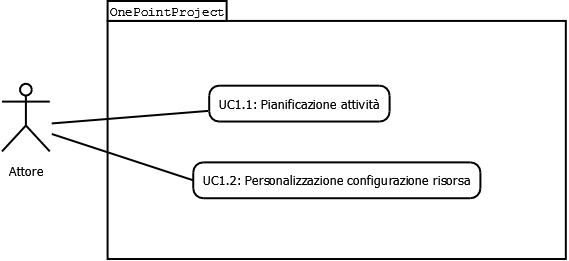
\includegraphics[width=0.80\textwidth]{img/UC/UC1.png}
\caption{UC1: Scenario principale}
\label{fig:UC1}
\end{center}
\end{figure}

\begin{description}
\item[Attori:]{utente autenticato al sistema.}
\item[Precondizione:]{Le infrastrutture di rete sono funzionanti e l\textquoteright{}applicativo \`{e} stato corretamente avviato.}
\item[Scenario principale:]{l\textquoteright{}utente pu\`{o} eseguire le seguenti operazioni:
	\begin{itemize}
	\item \textbf{pianificare le attivit\`{a}}: l\textquoteright{}utente dopo aver creato il progetto interessato o aperto in modifica uno esistente pu\`{o} utilizzare come strumento di pianificazione il WBS (UC1.1);
	\item \textbf{personalizzare la configurazione di una risorsa}: l\textquoteright{}utente accedendo al pannello di amministrazione risorse pu\`{o} scegliere come configurare una risorsa in termine di costi, sia interni che esterni, e di fascie orarie di lavoro e non (UC1.2).
	\end{itemize}}
\item[Postcondizione per successo:]{il sistema \`{e} in attesa di una scelta da parte dell\textquoteright{}utente.}
\end{description}

\subsubsection[UC1.1: Pianificazione attivit\`{a}]{UC1.1: Pianificazione attivit\`{a}}
\begin{figure}[H]
\begin{center}
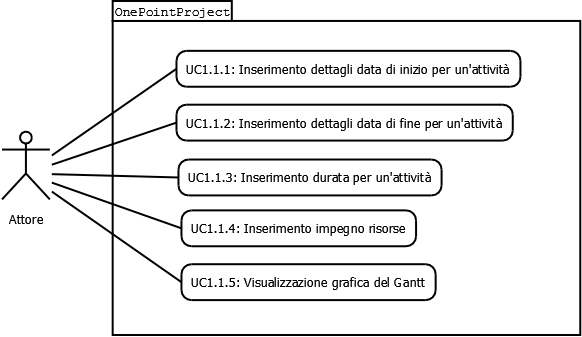
\includegraphics[width=0.80\textwidth]{img/UC/UC1.1.png}
\caption{UC1.1: Pianificazione attivit\`{a}}
\label{fig:UC1.1}
\end{center}
\end{figure}

\begin{description}
\item[Attori:]{utente autenticato al sistema.}
\item[Precondizione:]{L\textquoteright{}utente \`{e} in opzione modifica per un certo progetto e le infrastrutture di rete sono funzionanti.}
\item[Scenario principale:]{l\textquoteright{}utente pu\`{o} eseguire le seguenti operazioni:
	\begin{itemize}
	\item \textbf{inserire i dettagli relativi alla data di inizio dell\textquoteright{}attivit\`{a}}: l\textquoteright{}utente pu\`{o} inserire data e ora di inizio per un\textquoteright{}attivit\`{a} (UC1.1.1);
	\item \textbf{inserire i dettagli relativi alla data di fine dell\textquoteright{}attivit\`{a}}: l\textquoteright{}utente pu\`{o} inserire data e ora di fine per un\textquoteright{}attivit\`{a} (UC1.1.2);
	\item \textbf{inserire una durata per l\textquoteright{}attivit\`{a}}: l\textquoteright{}utente pu\`{o} inserire la durata dell\textquoteright{}attivit\`{a} nel formato dd-hh-mm che aggiorner\`{a} di conseguenza la data di fine, si tratta di un\textquoteright{}opzione alternativa all\textquoteright{}inserimento della data di fine (UC1.1.3);
	\item \textbf{inserire l\textquoteright{}impegno per le risorse coinvolte}: l\textquoteright{}utente dopo aver assegnato le risorse all\textquoteright{}attivit\`{a} interessata pu\`{o} scegliere le ore di lavoro della risorsa per l\textquoteright{}attivit\`{a} stessa (UC1.1.4);
	\item \textbf{visualizzazione del diagramma di Gantt}: l\textquoteright{}utente pu\`{o} visualizzare il diagramma di Gantt delle attivit\`{a} elencate nel WBS (UC1.1.5).
	\end{itemize}}
\item[Postcondizione per successo:]{il sistema aggiorna il WBS delle attivit\`{a} e in caso di salvataggio rende persitente la pianificazione effettuata.}
\end{description}

\subsubsection[UC1.2: Personalizzazione configurazione risorsa]{UC1.2: Personalizzazione configurazione risorsa}
\begin{figure}[H]
\begin{center}
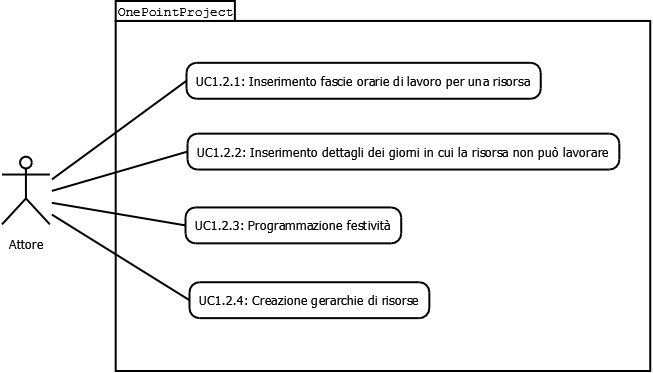
\includegraphics[width=0.80\textwidth]{img/UC/UC1.2.png}
\caption{UC1.2: Personalizzazione configurazione risorsa}
\label{fig:UC1.2}
\end{center}
\end{figure}

\begin{description}
\item[Attori:]{utente autenticato al sistema.}
\item[Precondizione:]{L\textquoteright{}utente ha i permessi per effettuare le modifiche alle risorse, ha quindi facolt\`{a} di accesso al pannello di amministrazione risorse e le infrastrutture di reste sono funzionanti.}
\item[Scenario principale:]{l\textquoteright{}utente pu\`{o} eseguire le seguenti operazioni:
	\begin{itemize}
	\item \textbf{inserire fascie orarie di lavoro per una risorsa}: l\textquoteright{}utente pu\`{o} inserire data e ora di inizio per un\textquoteright{}attivit\`{a} (UC1.2.1);
	\item \textbf{inserire i dettagli dei giorni in cui la risorsa \`{e} in stallo}: l\textquoteright{}utente pu\`{o} inserire data e facie orarie in cui la risorsa non pu\`{o} lavorare, pu\`{o} inoltre specificare le ragioni per cui la risorsa non pu\`{o} lavorare per esempio: manutenzione, locata a terzi ecc. (UC1.2.2);
	\item \textbf{programmare le festivit\`{a}}: l\textquoteright{}utente pu\`{o} indicare se una risorsa lavora o meno nei giorni festivi in base al calendario italiano (UC1.2.3);
	\item \textbf{creazione gerarchie di risorse}: l\textquoteright{}utente pu\`{o} specificare delle gerarchie di risorse tale che per una risorsa figlio \`{e} impostabile la possibilit\`{a} di ereditare o meno la configurazione del padre (UC1.2.4);
	\end{itemize}}
\item[Postcondizione per successo:]{il sistema aggiorna nel database le propriet\`{a} di configurazione delle risorse.}
\end{description}

\newpage

\section{OnePointProject}
\subsection{Architettura}
In questa sezione dar\`{o} una visione generale sull\textquoteright{}architettura dell\textquoteright{}applicativo. Il software presenta chiaramente una suddivisione in \textit{\textbf{macrocomponenti}}, ovvero l\textquoteright{}interfaccia grafica (View), la business logic (Model) e l\textquoteright{}application logic. L\textquoteright{}application logic riceve comandi dalla View e interagisce se necessario con gli altri \textit{\textbf{componenti}}. Il Model fornisce i metodi per accedere ai dati utili all\textquoteright{}applicazione. La View non interagisce in nessun modo con le componenti appartenenti al Model, ma solo con interfacce appartenenti alle componenti dell\textquoteright{}application logic. Il macrocomponente che presenta pi\`{u} sottocomponenti \`{e} l\textquoteright{}application logic; questo presenta classi di servizio e classi che effettuano operazioni logiche. Parte dei controlli sull\textquoteright{}inserimento dei dati da parte dell\textquoteright{}utente sono gestiti dalla View. Ogni elemento appartenente alla View eredita da una classe chiamata \textit{XView.java}; i principali elementi grafici: label, textbox, tabelle, \textit{\textbf{form}} appartengono tutti alla stessa classe, \textit{XComponent.java}; un \textit{\textbf{oggetto}} di tipo \textit{XComponent} presenta tra gli \textit{\textbf{attributi}} un campo di tipo stringa che ne indica il tipo; l\textquoteright{}applicativo presenta dei file di tipo \textit{\textbf{XML}} in cui viene definita la struttura di ogni form; i file che rappresentano la View vengono caricati dinamicamente al fine di eseguirne il parser e creare quindi gli oggetti di tipo \textit{XComponent} necessari. Nella struttura vengono definiti anche i nomi degli eventi che verrano invocati, ovvero i metodi che si occupano di gestire le operazioni dell\textquoteright{}utente. Lo svantaggio principale \`{e} l\textquoteright{}assenza di uno schema di riferimento da seguire per creare file che definiscono la struttura della View. Gli eventi vengono gestiti da degli script: nel momento in cui viene creato un oggetto di tipo \textit{XComponent}, ad esso vengono registrati se richiesto gli eventi; il comportamento di OnePointProject, d'ora in poi OPP, al verificarsi di un evento \`{e} il seguente: intercettazione dell\textquoteright{}evento da parte della classe, \textit{XInterpreter.java}, questa si occupa di richiamare il file di script indicato dall\textquoteright{}evento. Un file di script ha estensione \textit{jes}, contiene dei metodi e del codice Java, non contiene indicazioni in merito ai tipi dell\textquoteright{}oggetto, quindi se si invocano metodi su una certa variabile si deve assumere che quella variabile sia del tipo giusto. La funzione principale di questi script consiste in operazioni di recupero dati e di controllo. Gli script vengono interpretati da un compilatore ad hoc definito da OPP che richiama alla fine azioni eseguite da classi \textit{Java}. I file di script che necessitano operazioni di caricamento di nuovi form o operazioni che necessitano interazioni con il database invocano una richiesta inglobata in un oggetto di tipo \textit{XMessage} che ha come attributi il nome del servizio da invocare, il rispettivo \textit{\textbf{metodo}} e eventualmente i parametri necessari richiesti dalla \textit{\textbf{firma}} del metodo richiesto. Concludendo l\textquoteright{}applicativo presenta una struttura le cui modifiche in aggiunta non sono difficili da sviluppare, ma richiedono tempo per la loro integrazione con gli altri componenti. 

\subsection{Database}
L\textquoteright{}applicativo per relazionarsi con il database utilizza \textit{\textbf{Hibernate}}. Il file di mapping viene creato in modo automatico utilizzando dei file XML. L\textquoteright{}applicativo predisponde dei file XML per ogni classe i cui oggetti \`{e} necessario rendere persistenti. Questi file purtroppo non hanno uno schema predefinito da seguire e quindi obbligano il programmatore estraneo al team di sviluppo ad attenersi ai file gi\`{a} presenti in caso di modifiche o aggiunte da parte di quest\textquoteright{}ultimo. Il tutto \`{e} molto comodo, ma il principale svantaggio di questa scelta implementativa \`{e} che le classi Java presentano delle dipendenze cicliche. Tra breve dar\`{o} una spiegazione a riguardo; in OPP possono presentarsi tre casi, che ora illustrer\`{o}.

\subparagraph{Attributo il cui tipo non \`{e} definito dall\textquoteright{}utente} \quad \quad \\ \\
La sintassi da utilizzare sar\`{a} la seguente: \\
\textit{<field name=''Nome\_attributo'' type=''Tipo\_attributo''/>}; \\
Per esempio se nella classe \`{e} presente la dichiarazione: \textit{private String nome}, sar\`{a} sufficiente riportare nel file XML: \\
\textit{<field name=''nome'' type=''String''/>}.

\subparagraph{Attributo il cui tipo \`{e} un tipo composto} \quad \quad \\ \\
Si tratta di un tipo utilizzato per raccogliere un certo numero di attributi di tipo semplice, ad esempio \`{e} il caso dell\textquoteright{}indirizzo. Per esempio una classe dichiara una variabile di tipo \textit{Indirizzo}, che presenta i seguenti attributi di tipo semplice: \textit{via, numero civico, paese}.
La sintassi da utilizzare sar\`{a} la seguente:\\
\textit{<composite name=''nome attribuito al tipo composto'' type=''tipo della classe composta''>} \\
\textit{<field name=''Nome attributo java'' column=''Nome attributo colonna nel database'' type=''Tipo dell\textquoteright{}attributo''/>} \\
\textit{</composite>}.\\
Ovviamente, e questo vale per tutte le casistiche, il \textit{\textbf{tag}} field pu\`{o} essere accompagnato dall\textquoteright{}impostazione di alcune propriet\`{a}, ad esempio se l\textquoteright{}attributo deve essere richiesto o meno nel db \textit{(mandatory=``true\textquoteright{}\textquoteright{})}, se l\textquoteright{}attributo deve essere ordinabile \textit{(ordered=''true'')} ecc. Nel database tutti gli attributi del tipo composto sono inglobati come attributi della tabella nella cui classe \`{e} stata indicata una dipendenza nei confronti del tipo composto, non verr\`{a} quindi realizzata una tabella a se stante rappresentante l\textquoteright{}entit\`{a} del tipo composto.

\subparagraph{Relazioni tra entit\`{a}} \quad \quad \\ \\
Si ha quindi una dipendenza tra tipi, nel database viene espressa con relazioni del tipo \textit{1:1, 1:n, m:n}. Le relazioni \textit{m:n} vengono scomposte in 2 relazioni di tipo \textit{1:n} introducendo una nuova relazione. A questo corrisponde anche una classe Java, in questo modo ad ogni relazione corrisponder\`{a} sempre una classe Java.\\
Riporto qui un esempio del tipo di relazione in questione: \\
nella classe \textit{OpActivity.java} si ha la seguente dichiarazione: \textit{private OpProjectPlan projectplan}; nel file XML corrispondente alla classe OpActivity.java \`{e} presente il seguente tag: \\
\textit{<relationship name=''ProjectPlan'' type=''OpProjectPlan'' back-relationship=''Activities''/>}
Quindi occorre indicare il nome dell\textquoteright{}attributo, il tipo e la relazione; nel file XML corrispondente alla classe OpProjectPlan.java \`{e} definito un tag che a seconda del tipo di relazione \textit{1:1 o 1:n} sar\`{a} rispettivamente: \\
\textit{<relationship name=''Activities'' type=''OpActivity'' back-relationship=''ProjectPlan''/>}, oppure \\
\textit{<relationship name=''Activities'' type=''OpActivity'' collection-type=''Set'' \\ back-relationship=''ProjectPlan'' cascade=''delete''/>}.\\
L\textquoteright{}attributo name si deve riferire ad un attributo della classe Java corrispondente; in questo modo si presentano delle dipendenze cicliche. La classe \textit{OpProjectPlan.java} presenta un attributo che \`{e} una collezione di oggetti di tipo \textit{OpActivity} e la classe \textit{OpActivity.java} presenta un riferimento all\textquoteright{}oggetto di tipo \textit{OpProjectPlan} corrispondente. Questo scelta potrebbe portare a delle inconsistenze di dati a \textit{\textbf{run-time}}.

\begin{figure}[H]
\begin{center}
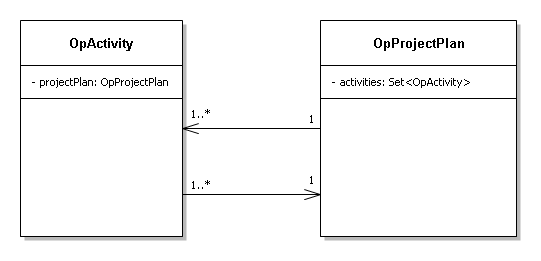
\includegraphics[width=1\textwidth]{img/DipendenzaCiclica.png}
\caption{Esempio di dipendenza ciclica}
\label{fig:Esempio di dipendenza ciclica}
\end{center}
\end{figure}

\newpage

\section{Progettazione}
In questa sezione viene data la specifica di quello che \`{e} stato progettatto per ogni incremento, utilizzando un linguaggio discorsivo in cui si spiegano le ragioni e le situazioni che hanno portato a determinate scelte progettuali.
\subsection{Incremento 1}
Il primo incremento consiste nell\textquoteright{}introduzione nella pianificazione delle attivit\`{a} nel riportare il loro inizio e fine alla precisione del minuto. Questa parte di progettazione viene tracciata con il soddisfacimento dei seguenti requisiti:

\begin{longtable}{|>{\centering}p{3cm}|}
    \hline
    \multicolumn{1}{|c|}{\textbf{Requisiti}} \\ %\tabularnewline 
      \hline
        RF.ob.1 \tabularnewline \hline
		RF.ob.1.1 \tabularnewline \hline
		RF.ob.1.2 \tabularnewline \hline
		RF.ob.2 \tabularnewline \hline
		RF.ob.3 \tabularnewline \hline
    \caption{Tracciamento requisiti - Componenti incremento1}
    \label{tab:Tracciamento requisiti - Componenti incremento1}
\end{longtable}

Le classi appartenenti al Model, che memorizzano le informazioni relative alla data di inizio e fine utilizzano, alla versione di OnePointProject scaricabile da sourceforge, un tipo \textit{java.sql.Date}; tuttavia nel database MsSQL la data di inizio e fine vengono salvate con un tipo \textit{datetime}. Quindi per questo incremento \`{e} stato scelto di cambiare il tipo \textit{java.sql.Date} con il tipo \textit{java.sql.Timestamp}, per le seguenti ragioni: data e ora memorizzate in un solo campo del database; data e ora memorizzate in un solo tipo Java; poich\`{e} l\textquoteright{}applicativo nel diagramma di Gantt utilizza per le operazioni la trasformazione della data in millisecondi \`{e} pi\`{u} facile adattare le modifiche cambiando il tipo in un tipo che presenta lo stesso metodo per ottenere i millisecondi. Quindi in questo modo il diagramma di Gantt per durate di attivit\`{a} superiore al giorno visualizzer\`{a} le attivit\`{a} nella posizione corretta rispetto all\textquoteright{}ora del giorno impostato. In questa fase occorrono anche delle modifiche da apportare ai form per l\textquoteright{}inserimento di attivit\`{a} in WBS, permettendo l\textquoteright{}inserimento dell\textquoteright{}ora di inizio e fine oltre che la data; occorre cambiare il tipo di inserimento della durata; il tipo progettato ha nominativo \textit{durationstring}. Per questo nuovo tipo occorre seguire la seguente procedura:
\begin{description}
\item[XComponent.java]: aggiungere \textit{case} per la visualizzazione del componente, per l\textquoteright{}impostazione del valore, per l\textquoteright{}impostazione del tipo di editor, per gli eventi che vedono coinvolto il componente.
\item[XExpressProxy.java]: questa classe svolge la funzione di proxy di protezione per l\textquoteright{}interazione tra file di script (con estensione \textit{jes}) e i metodi delle classi \textit{Java} interessate. In questa classe \`{e} necessario aggiungere i metodi che coinvolgono il tipo interessato. Nel caso del tipo \textit{durationstring} sono stati progettati metodi di set e get del valore che il tipo racchiude.
\item[XDefaultComponentHandler]: questa classe viene utilizzata come classe di \textit{''factory''} per i vari componenti grafici in relazione al tipo; occorre aggiungere il \textit{case} per la creazione di oggetti \textit{XComponent} di tipo \textit{durationstring}.
\end{description}

\subsection{Incremento 2}
Il secondo incremento consiste nella creazione dei componenti necessari per la configurazione delle risorse. Questa parte di progettazione viene tracciata con il soddisfacimento dei seguenti requisiti:

\begin{longtable}{|>{\centering}p{3cm}|}
    \hline
    \multicolumn{1}{|c|}{\textbf{Requisiti}} \\ %\tabularnewline 
      \hline
        RF.ob.5 \tabularnewline \hline
		RF.ob.5.1 \tabularnewline \hline
		RF.ob.5.1.1 \tabularnewline \hline
		RF.ob.5.1.2 \tabularnewline \hline
		RF.ob.5.2 \tabularnewline \hline
		RF.ob.5.3 \tabularnewline \hline
		RF.ob.5.4 \tabularnewline \hline
		RF.ob.5.4.1 \tabularnewline \hline
    \caption{Tracciamento requisiti - Componenti incremento2}
    \label{tab:Tracciamento requisiti - Componenti incremento2}
\end{longtable}

Nello sviluppo di questo incremento \`{e} necessario integrare componenti alla View, al Model e all\textquoteright{}application logic.
In OnePointProject alla versione presa in modifica \`{e} presente un pannello di amministrazione risorse in cui \`{e} possibile impostare i costi interni o esterni per la risorsa. Al pannello in questione \`{e} stato progettata l\textquoteright{}aggiunta di nuove schede per l\textquoteright{}inserimento dei dati richiesti dai requisiti tracciati per questo incremento. Le schede da aggiungere sono 3: una per l\textquoteright{}inserimento delle fascie orarie in cui la risorsa pu\`{o} lavorare con la relativa opzione di ereditarit\`{a} delle fascie orarie dal padre per rispettare i vincoli gerarchici; una per l\textquoteright{}inserimento dei giorni in cui la risorsa non pu\`{o} lavorare e le relative fascie orarie con l\textquoteright{}opzione di ereditariet\`{a} dei giorni e delle fascie di fermo dalla risorsa padre; infine una scheda in cui si pu\`{o} impostare se la risorsa lavori o meno nei giorni festivi. Per le modifiche grafiche \`{e} sufficiente modificare il file \textit{edit\_resource.oxf.xml}.
Nel form in cui vanno inserite le disponibilit\`{a} delle fascie orarie delle risorse \`{e} presente una tabella dalla quale \`{e} possibile effettuare l\textquoteright{}aggiunta di una fascia oraria o rimuovere una fascia selezionata. La gestione degli eventi per questo form \`{e} stata impostata in modo che essa venga attuata direttamente da una classe Java e non da un file di script, si tratta dell\textquoteright{}unico form gestito da OnePoint con la normale procedura; la classe in questione \`{e} \textit{OpEditResourceFormHandler.java}. A questa occorre aggiungere tutti i metodi per la gestione degli eventi ed \`{e} necessario gestire il caso in cui si ha la sovrapposizione di intervalli, ovvero fascie orarie inserite dall\textquoteright{}utente. Analogo \`{e} il comportamento della gestione della scheda per l\textquoteright{}inserimento delle fascie orarie in cui la risorsa \`{e} bloccata, con eccezione del fatto che \`{e} possibile impostare anche il giorno in cui la risorsa \`{e} bloccata. L\textquoteright{}utente pu\`{o} inserire pi\`{u} giorni in cui la risorsa \`{e} impossibilitata nel suo lavoro, il sistema non deve comunque rendere persistenti i dati fino a quando non viene effettuato il salvataggio; quindi \`{e} necessario predisporre in \textit{OpEditResourceFormHandler.java} un campo statico con la seguente firma:\\ \textit{public static Map<Timestamp,XComponent> mappaCalendario}; \\ ovvero la chiave sar\`{a} la data scelta e il valore sar\`{a} un set che rappresenta le fascie orarie; l\textquoteright{}inizializzazione va fatta nel momento in cui viene aperto il form per la gestione di una certa risorsa e tale mappa andr\`{a} inizialmente caricata con i dati presenti nel databasee. La mappa andr\`{a} aggiornata nel momento in cui si cambia data e/o vengono fatte aggiunte e/o rimozioni di fascie orarie. Anche il Model \`{e} stato modificato, in particolare \`{e} stato modificato \textit{OpResource.java}, per maggior chiarezza riporto qui la nuova struttura per rappresentare la risorsa interessata.

\begin{figure}[H]
\begin{center}
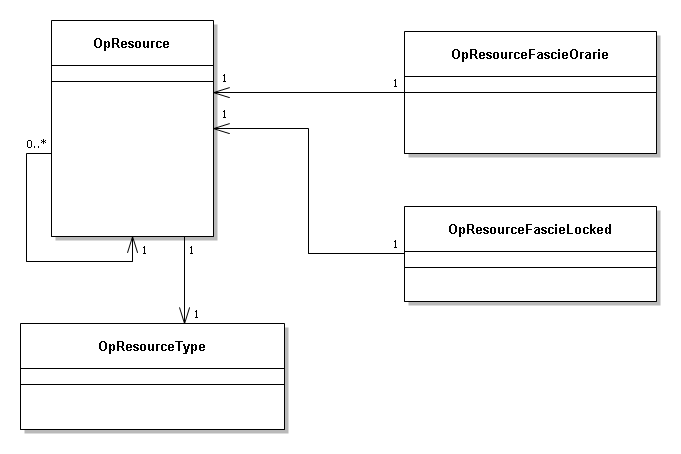
\includegraphics[width=1\textwidth]{img/Resource.png}
\caption{Model: sottocomponente risorsa}
\label{fig:Model: sottocomponente risorsa}
\end{center}
\end{figure}

La seguenta tabella rappresenta i principali attributi caratteristici di una risorsa:
\begin{tabbing}
TABLE \=op\_resource (\\
\>    op\_resourcepool bigint,\\
\>    op\_site bigint,\\
\>    op\_archived bit DEFAULT (0),\\
\>    op\_inheritpoolrate bit,\\
\>    op\_hourlyrate numeric(22, 10),\\
\>    op\_externalrate numeric(22, 10),\\
\>    op\_description varchar(2500),\\
\>    op\_user bigint,\\
\>    op\_inheritfestivita bit, *\\
\>    op\_festivita bit, *\\
\>    op\_inheritfascieorarie bit, *\\
\>    op\_inheritfascielocked bit *,\\
\>    op\_typeresource *\\
);
\end{tabbing}
\textbf{*= add by me} \\ \\
Una risorsa appartiene ad una gerarchia di risorse identificata dall\textquoteright{}attributo op\_resorcepool, che \`{e} una risorsa stessa. Quindi nella relazione sono presenti degli attributi \textit{boolean} (di tipo \textit{bit} in MS Sql) che indicano se l\textquoteright{}entit\`{a} interessata (la risorsa) eredita o meno dalla risorsa padre. Una risorsa pu\`{o} ereditare dal padre i costi, la festivit\`{a}, le fascie orarie, gli impegni della risorsa.
Una risorsa per OnePointProject \`{e} indifferente dal tipo, cio\`{e} una risorsa umana si comporta come una risorsa strumentale. Per CQT e VIDA no, quindi \`{e} stato predisposto un campo op\_resourcetype che si riferisce a una tabella che accumula i tipi della risorsa disponibile.
L\textquoteright{}aggiunta di un tipo comporta un aggiustamento del calcolo. Per ora il calcolo viene effettuatato considerando risorse umane e strumentali.

\subsection{Incremento 3}
Il terzo incremento prevede la gestione del calcolo della durata delle attivit\`{a} in relazione al WBS pianificato. Questa parte di progettazione viene tracciata con il soddisfacimento dei seguenti requisiti:

\begin{longtable}{|>{\centering}p{3cm}|}
    \hline
    \multicolumn{1}{|c|}{\textbf{Requisiti}} \\ %\tabularnewline 
      \hline
        RF.ob.4 \tabularnewline \hline
		RF.ob.4.1 \tabularnewline \hline
		RF.ob.4.1.1 \tabularnewline \hline		
		RF.ob.4.1.1.1 \tabularnewline \hline
		RF.ob.4.1.1.2 \tabularnewline \hline
		RF.ob.4.1.1.3 \tabularnewline \hline
		RF.ob.4.1.2 \tabularnewline \hline
		RF.ob.4.1.2.1 \tabularnewline \hline
		RF.ob.4.1.2.2 \tabularnewline \hline
		RF.ob.4.1.2.2.1 \tabularnewline \hline
		RF.ob.4.1.2.2.2 \tabularnewline \hline
		RF.ob.4.1.3 \tabularnewline \hline
    \caption{Tracciamento requisiti - Componenti incremento3}
    \label{tab:Tracciamento requisiti - Componenti incremento3}
\end{longtable}

Il calcolo viene effettuato nel momento in cui l\textquoteright{}utente decide di effettuare un\textquoteright{}operazione di salvataggio. Viene effettuato, quindi eventualmente aggiornato nel momento in cui, viene cambiata la data di inizio\/fine di un\textquoteright{}attivit\`{a}, quindi la durata, oppure nel momento in cui viene fatta una modifica agli assegnamenti delle attivit\`{a}, modificandoli eliminandoli o inserendone di nuovi. Per fare ci\`{o} nel pi\`{u} semplice modo possibile occorre aggiungere al metodo di salvataggio gi\`{a} previsto dall\textquoteright{}applicativo il metodo con la seguente firma \\
\textit{eseguiCalcolo(OpBroker broker,OpProjectSession session,OpProjectPlanVersion project);} \\
Un oggetto di tipo \textit{OpBroker} viene utilizzato quando sono necessarie operazioni con il database; la classe \textit{OpBroker.java} presenta metodi per effettuare query e operazioni di CRUD su ennuple e quindi su oggetti. Un oggetto di tipo \textit{OpProjectSession} \`{e} necessario per aprire transazioni e svolge il ruolo di sessione vera e propria ovvero identifca l\textquoteright{}utente autenticato al sistema. Un oggetto di tipo OpProjectPlanVersion al fine di identificare il progetto in modifica, con un diagramma delle classi cercher\`{o} di spiegare la funzionalit\`{a} delle classi che riportano alla fine del nome la parola \textit{''Version''}.

\begin{landscape}
\begin{figure}[H]
\begin{center}
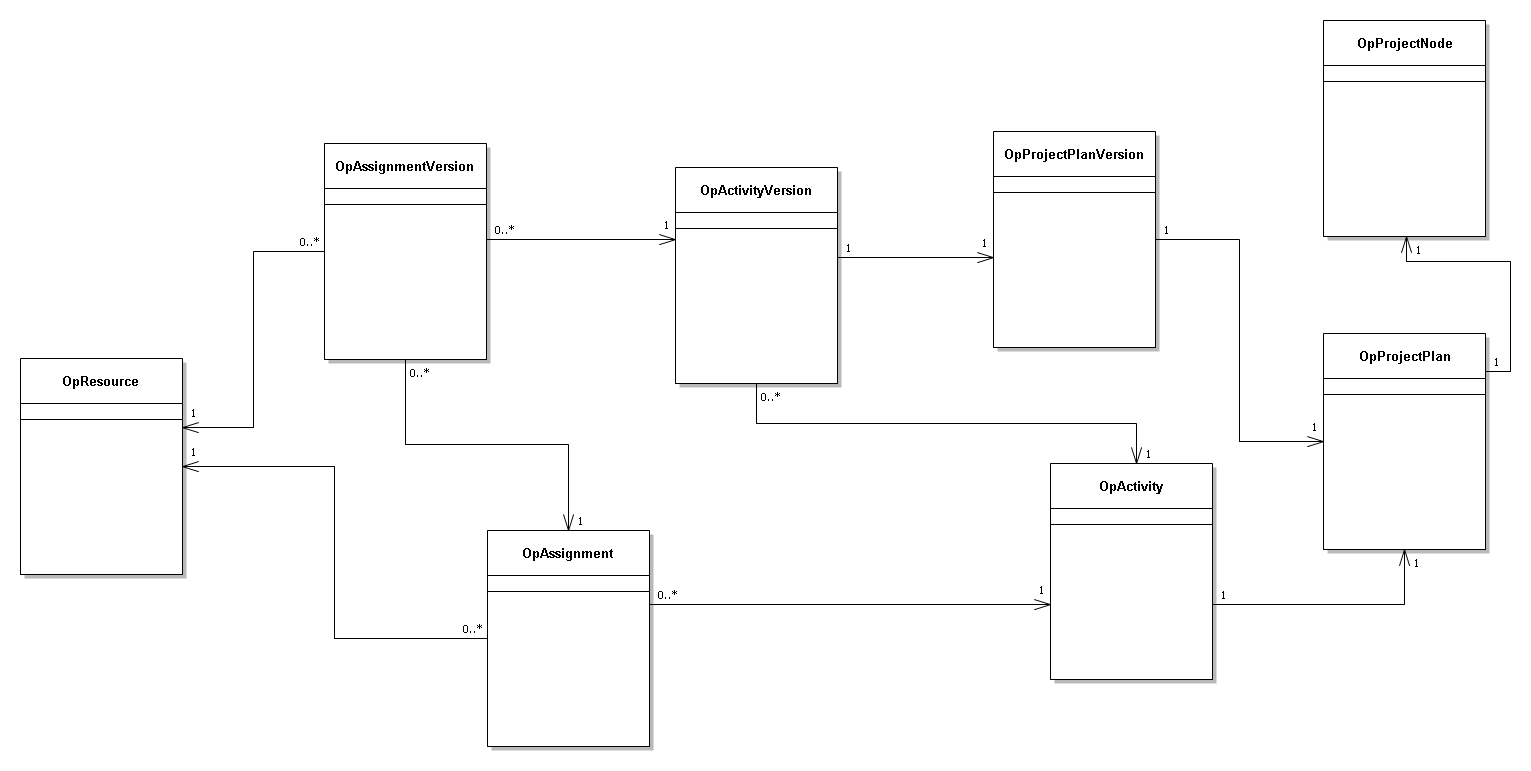
\includegraphics[width=1.6\textwidth]{img/ModelIncremento2.png}
\caption{Model: sottocomponente versionamento}
\label{fig:Model: sottocomponente versionamento}
\end{center}
\end{figure}
\end{landscape}.

Il versionamento delle attivit\`{a} non funziona come un repository. La funzionalit\`{a} \`{e} quella di rendere visibili a tutti le informazioni del progetto all\textquoteright{}ultimo ''check-in'' effettuato, in questo modo se un utente sta modificando il progetto le sue modifiche non verranno viste da tutti fino al suo prossimo ''check-in''. In pratica si tratta di lock in scrittura e la lettura \`{e} permessa all\textquoteright{}ultima versione per cui \`{e} stato fatto il ''check-in''.
Nel momento in cui viene effettuata una operazione di salvataggio viene creato un oggetto di tipo \textit{OpActivityVersion} o al massimo esso viene aggiornato, sempre all\textquoteright{}ultima versione ovviamente. Quando si effettua il ''check-in'' viene a crearsi un oggetto di tipo \textit{OpActivity}, che \`{e} la copia di ci\`{o} che \`{e} riportato in \textit{OpActivityVersion} all\textquoteright{}ultima versione del piano di progetto.
Un oggetto di tipo \textit{OpProjectPlan} viene creato nel momento in cui si crea un oggetto di tipo \textit{OpProjectNode}, quindi esister\`{a} sempre almeno un oggetto di tipo \textit{OpProjectPlan} riferito al nuovo progetto. Nel momento in cui si salvano le prime attivit\`{a} si crea anche un oggetto di tipo \textit{OpProjectPlanVersion}. Il versionamento \`{e} previsto anche per gli assegnamenti delle risorse alle attivit\`{a}, quindi \`{e} presente una classe \textit{OpAssignment} e una classe \textit{OpAssignmentVersion}.


\subsection{Incremento 4}
Il quarto incremento consiste nella possibilit\`{a} di modificare graficamente il diagramma di Gantt e di apportare modifiche al WBS nel caso in cui venga modificata la durata delle attivit\`{a} del diagramma di Gantt, con incrementi o decrementi di durata inferiore alle 24 ore. Questa parte di progettazione viene tracciata con il soddisfacimento dei seguenti requisiti:

\begin{longtable}{|>{\centering}p{3cm}|}
    \hline
    \multicolumn{1}{|c|}{\textbf{Requisiti}} \\ %\tabularnewline 
      \hline
        RF.de.1 \tabularnewline \hline
		RF.de.2 \tabularnewline \hline
		RF.de.3 \tabularnewline \hline
		RF.de.3.1 \tabularnewline \hline
		RF.de.3.2 \tabularnewline \hline
    \caption{Tracciamento requisiti - Componenti incremento4}
    \label{tab:Tracciamento requisiti - Componenti incremento4}
\end{longtable}
\newpage

\section{Processi di revisione adottati}
Per il progetto sono state fissate delle milestone al termine delle quali � stata concordata un'operazione di controllo. L'introduzione delle revisioni nel piano di progetto � stata fatta in accordo agli standard aziendali, anche se dall'azienda sono eseguite settimanalmente piuttosto che alla fine di milestone precise. Ogni revisione � stata svolta nella sala riunioni dell'azienda in cui sono presenti un proiettore, una lavagna, un tavolo, e dei computer; lo strumento che � stato deciso di utilizzare � il proiettore, quindi la milestone doveva concludere con la realizzazione di una presentazione in cui figuravano i contenuti essenziali.\\
La prima revisione � stata eseguita al termine della fase di lavoro in comune; in questa revisione sono stati divisi i contenuti tra me e il collega stagista Petrin; in questa revisione sono state spiegate le scelte implementative di OPP, note all'azienda solo parzialmente e questa almeno da parte mia � stata una sorpresa nel senso che il programma nel dettaglio non era conosciuto, ma � stato scelto come la miglior soluzione che l'azienda potesse adottare e quindi adattare ai requisiti. OPP in realt� essendo privo di documentazione, da quello che ho potuto sperimentare richiede tempo nelle modifiche da applicare, proprio perch� non conoscendo dall'inizio le componenti da modificare occore identificarle, ma non sempre si riesce a identificarle tutte fin dall'inizio e quindi nello sviluppo si arriva ad uno stato incerto che potrebbe rivedere delle modifiche alla progettazione. Questo fatto � stato presentato all'azienda, ma non gli � stata data molta importanza. \\
Alla seconda revisione sono stati presentati per la parte relativa al mio progetto i casi d'uso al fine di chiarire se avevo compreso quello che il software doveva realizzare; questa revisione � stata molto utile perch� a me sono stati chiariti dei punti un p� oscuri, mentre l'azienda ha riflettuto meglio sul da farsi e ha mosso dei ticket in cui venivano applicate delle modifiche e aggiunte ai requisiti previsti. Lo strumento dei casi d'uso con UML non � applicato dall'azienda, ma lo ha trovato utile e intuitivo. \\
La terza revisione � stata complessa da presentare, per il fatto che le scelte progettuali richiedevano per la maggior parte la modifica di metodi gi� sviluppati. La presentazione � stata divisa in 3 parti:
\begin{description}
\item nella prima parte venivano indicate le componenti che l'applicativo non presentava e che dovevano essere aggiunte;
\item nella seconda parte sono state presentate le classi e i rispettivi metodi che richiedavano modifiche nel contenuto o nella firma; una modifica della firma presentava una catena di altre modifiche per tutte le classi che si interfacciavano con il metodo da modificare, per questa ragione le modifiche di questo tipo di questo tipo si � cercato di ridurle al massimo;
\item alla fine � stato presentato il tracciamento componenti-requisiti in cui veniva specificata la ragione che ha portato a quel tipo di progettazione.
\end{description}

L'ultima revisione coincideva con l'accettazione del software. A questa revisione � stata presentata la qualifica del prodotto, o meglio gli esiti dei test eseguiti, e l'esecuzione dei test di sistema. L'esito complessivo � stato per l'azienda soddisfacente.
\newpage

\section{Programmazione}
In questa sezione vengono elencati gli stumenti di sviluppo, le regole e le procedure stabilite per codificare ci� che � stato previsto dalla progettazione.

\subsection{Strumenti di sviluppo}
L'azienda ha imposto e predisposto l'installazione di Eclipse Juno; questo pu� essere utilizzato per la produzione di software di vario genere fornendo un completo IDE per il linguaggio Java. La piattaforma di sviluppo � incentrata sull'uso di plug-in che possono essere da chiunque sviluppati. Alla versione installata � stato aggiunto il plug-in Eclipse Subversive, al fine di versionare il codice. Il repository � stato creato sui server aziendali. Sullo stesso sono stati aggiunti anche i documenti tecnici sviluppati durante la fase di manutenzione.

\subsection{Procedure}
Per la codifica � stata seguita la seguente procedura:
\newcommand{\circleditem}[1]{\tikz[baseline=-0.4em] \draw node[draw,circle,inner sep=0,align=center] {\scriptsize \makebox[3mm]{#1}};}
\begin{enumerate}[label=\protect\circleditem{\theenumi}]
\item ciclare sugli incrementi progettati;
\item debugging per identificare le componenti che si integrano con l'incremento pianificato e progettato;
\item codifica;
\item test di unit�;
\item applicazione di commenti al codice;
\item riportare nel changelog le modifiche applicate.
\end{enumerate}
A incremento codificato � necessario procedere con i test di integrazione. Non essendo stata comunicata una prassi aziendale riguardante la documentazione del codice si sono scelti i seguenti metodi di documentazione:
\begin{itemize}
\item \textbf{commenti interni al codice}: le righe di codice che potrebbero risultare di comprensione non intuitiva o di una certa complessit� devono essere commentate, fornendo dettagli tecnici;
\item \textbf{architettura di dettaglio}: oltre all'identificazione delle classi da modificare e ai diagrammi delle classi relativi alle integrazioni occorre fornire una documentazione sui metodi da implementare munendoli di firma e di una descrizione sulle funzionalit� che essi compiono.
\end{itemize}


Procedura di modifica architettura:
\begin{enumerate}[label=\protect\circleditem{\theenumi}]
\item modifica classi Model;
\item modifica file con estensione *.opt.xml al fine di aggiornare le relazioni del database;
\item modifica dei file con estensione *.oxf.xml al fine di modificare le View necessarie;
\item modifica dei file di script che gestiscono gli eventi;
\item modifica delle classi Java, che svolgono la funzionalit� di handler degli eventi;
\item modifica dell'application logic.
\end{enumerate}


\subsection{Regole}
Le regole principali che sono state seguite sono le seguenti:
\begin{enumerate}[label=\protect\circleditem{\theenumi}]
\item in accordo con la progettazione non violare le dipendenze previste dall'architettura;
\item adottare il principio zero warnings;
\item limitare la complessit� ciclomatica ad un livello pari a 5;
\item il codice deve presentare l'indentazione adottata dall'applicativo;
\item 1 riga = 1 istruzione;
\item non violare regole di codifica adottate dall'applicativo.
\end{enumerate}
\newpage

\section{Test e collaudo}
\subsection{Strumenti e tecniche di verifica}
Gli strumenti utilizzati sono forniti da Eclipse; in particolare � stato pesantemente utilizzato il debugger, il quale facilita la visione dei contenuti delle varie strutture dati a tempo di esecuzione ed evidenzia per il test-case in questione i dati prodotti permettendo in caso di errore di indagare su quali componenti occorre applicare delle correzioni immediate o comunque da sottoporre a correzione in un momento successivo e in quest'ultimo caso segnalando un ticket attraverso uno strumento messo a disposizione dall'azienda \textit{RedMine}. Per la verifica sono state svolte le seguenti 2 tecniche:
\begin{itemize}
\item \textbf{analisi statica}: realizzata dagli strumenti di sviluppo utilizzati che evidenziano eventuali errori commessi, che il flusso di controllo possa essere raggiunto e che i dati non assumano valori illegali o senza senso;
\item \textbf{analisi dinamica}: sono stati pianificati i test di unit� per ogni metodo, indicando nel documento di qualifica del prodotto, identificativo del test e relativi esiti. Sono stati definiti i casi di prova per ogni metodo analizzando il codice dei metodi quindi sono stati effettuati test di tipo white-box, seguendo per ognuno il debugging. Per i metodi aggiunti dalla progettazione e dal debugging sono stati ricavati i flussi di dati e di chiamata al fine di integrare le componenti con la pi� scarsa possibilit� di errors; lo strumento utilizzato per lo svolgimento dei test di unit� e integrazinoe � stato JUnit. Le procedure di verifica hanno includevano la seguente checklist:
	\begin{enumerate}
	\item \textbf{verifica strutture dati}: sono state controllate le strutture dati utilizzate come tipo di ritorno di un metodo; sono stati controllati gli oggetti immagazzinati in iteratori, prevalentemente come risultato di query;
	\item \textbf{inserimento dei dati}: � stato verificata la corretta interazione del software con l'utente e il comportamento in caso di errori in inserimenti dati e il comportamento in caso di inserimenti corretti; � stato controllato anche l'inserimento dei dati nel database e il comportamento in caso di commit o rollback di transazioni;
	\end{enumerate}
\end{itemize}

\subsection{Collaudo finale}
\newpage

\section{Conclusioni}
Lo stage determina il passo intermedio tra la scuola e il mondo del lavoro e solo con questa esperienza o comunque altre attivit� lavorative � possibile integrarsi in questo ambiente. In questa esperienza, la prima presso un'azienda informatica, sono entrato in diretto contatto con le difficolt� che animano un'azienda quotidianamente. I problemi non sono strettamente di natura informatica, ma anche di gestione del personale e organizzazione del lavoro. La struttura dell'azienda non � predisposta per sviluppo di progetti, in modo tale quindi da dedicare le risorse alla sole attivit� di progetto; l'azienda � caratterizzata da risorse che alternano le mansioni di una risorsa dall'analisi allo sviluppo del software, dall'incontro con i clienti alla manutenzione di software ad essi venduti. Da questo ne ricavo che � indispensabile avere un'organizzazione delle risorse e dell'ambiente di lavoro al fine di fissare le funzionalit� competenti una deternminata risorsa, le responsabilit�, le procedure e le regole. Dallo stage ho appreso l'importanza delle conoscenze acquisite grazie all'universit�, ma ho soprattutto capito che la laurea � un traguardo importante, ma in questo settore ci� che vince � l'esperienza o meglio le best practice. Per quanto riguarda il progetto di stage sono rimasto soddisfatto del risultato ottenuto, inoltre la manutenzione di software ha come pregio la possibilit� di analizzare le scelte architetturali di altri team, permettendo quindi di valutare le scelte implementative, pensando a strategie diverse di sviluppo; il tutto per un laureando � molto utile perch� permette di imparare da altri puntando necessariamente al miglioramento continuo. Quindi la mia esperienza di stage si � alternata da fasi monotone di debugging, anche un po noiose, ma indispensabili per apprendere l'architettura del sofware a fasi di modifica dell'applicativo che hanno permesso di portare avanti il ciclo di vita del software di OPP.
\newpage

\pagestyle{stilecapitolinonnumerati}

\section*{Glossario}
Nel documento la prima occorrenza delle parole presenti nel glossario vengono evidenziate con la formattazione in grassetto e corsivo.\\ \\

\Huge A
\normalsize
\begin{itemize}
\item \textbf{ad hoc}: ovvero appropriato, specificatamente realizzato.
\item \textbf{attivit�}: organizzazione di compiti.
\item \textbf{attributi}: propriet� di una certa classe o tabella.
\end{itemize}

\Huge B
\normalsize
\begin{itemize}
\item \textbf{baseline}: pianificazione del software ad una certa versione.
\end{itemize}

\Huge C
\normalsize
\begin{itemize}
\item \textbf{componenti}: elemento definito con funzionalit�, responsabilit� e interfacce specifiche.
\item \textbf{CQT}: si tratta di un software prodotto dall'azienda RDS-NORDEST che � in fase di manutenzione.
\item \textbf{CRUD}: create,read,update and delete.
\item \textbf{check-in}: in OPP operazione che rende visibile a tutti gli utenti le modifiche effettuate su un determinato progetto.
\item \textbf{collection\_activity}: tipo definito in OPP per indicare un'attivit� che racchiude un sottoinsieme di sottoattivit� di tipo standard o collection.
\item \textbf{changelog}: registro delle modifiche.
\item \textbf{complessit� ciclomatica}: nota anche come complessit� di McCabe; si tratta di una metrica software utilizzata per misurare la complessit� di un programma; misura direttamente il numero di cammini linearmente indipendenti attraverso il grafo di controllo di flusso.
\item \textbf{commit}: esito positivo nell'esecuzione di una transazione che porta il database ad un nuovo stato.
\item \textbf{checklist}: lista di controllo ovvero un qualsiasi elenco esaustivo di cose da fare o da verificare per eseguire una determinata attivit�.
\end{itemize}

\Huge D
\normalsize
\begin{itemize}
\item \textbf{debugging}: attivit� che consiste nell'esecuzione del software guidata dal verificatore.
\item \textbf{dominio}: termine utilizzato nella fase di analisi dei requisiti per indicare l'ambiente con il quale il sistema deve integrarsi.
\end{itemize}

\Huge E
\normalsize
\begin{itemize}
\item \textbf{ennuple}: l'insieme dei valori in una tabella di un database.
\end{itemize}

\Huge F
\normalsize
\begin{itemize}
\item \textbf{form}: interfaccia che consente all'utente di inserire dati.
\item \textbf{firma}: prototipo del metodo.
\item \textbf{factory}: ovvero creato per la creazione di altri oggetti.
\end{itemize}

\Huge G
\normalsize
\begin{itemize}
\item \textbf{GDO}: ovvero grande distribuzione organizzata.
\item \textbf{Gantt}: il diagramma di Gantt � lo strumento pi� utilizzato tanto nella fase operativa, quanto in quella di controllo; si tratta di un diagramma cartesiano, ovvero, una rappresentazione grafica bidimensionale: sulle ascisse (lungo l'asse orizzontale) viene riportata la variabile temporale, mentre lungo le ordinate (asse verticale) soni indicate le attivit� nella quali � stato scomposto il progetto.
\end{itemize}

\Huge H
\normalsize
\begin{itemize}
\item \textbf{Ho.Re.Ca.}: azienda che si occupa della distribuzione di alimentari.
\item \textbf{Hibernate}: � una piattaforma middleware open source per lo sviluppo di applicazioni Java, attraverso l'appoggio al relativo framework, che fornisce un servizio di object-relational mapping (ORM) ovvero gestisce la persistenza dei dati sul database attraverso la rappresentazione e il mantenimento su database relazionale di un sistema di oggetti Java.
\end{itemize}

\Huge I
\normalsize
\begin{itemize}
\item \textbf{impegno}: indica lo sforzo assegnato ad una risorsa per una certa attivit�.
\item \textbf{IDE}: componente integrato a editor di testo utilizzata per fornire aiuti di sintassi al programmatore.
\item \textbf{iteratori}: un iteratore � un oggetto che consente di visitare tutti gli elementi contenuti in un altro oggetto, tipicamente un contenitore.
\end{itemize}

\Huge J
\normalsize
\begin{itemize}
\item \textbf{Java}: linguaggio di programmazione orientato agli oggetti.
\end{itemize}

\Huge K
\normalsize
\begin{itemize}
\item \textbf{know-how}: identifica le conoscenze e le abilit� operative necessarie per svolgere una determinata attivit� lavorativa.
\end{itemize}

\Huge L
\normalsize
\begin{itemize}
\item \textbf{LIMS}: software usato nei laboratori d'analisi per la gestione integrata di molteplici tipi di dati e processi.
\item \textbf{lock}: meccanismo di sincronizzazione per limitare l'accesso ad una risorsa condivisa.
\end{itemize}

\Huge M
\normalsize
\begin{itemize}
\item \textbf{milestone}: traguardi intermedi previsto nello svolgimento di un progetto; rappresenta un'attivit� con nome e durata pari a 0.
\item \textbf{macrocomponenti}: componente non terminale che � formato da sottocomponenti; termine utilizzato per dare una definizione di prodotto ad alto livello. 
\item \textbf{metodo}: operazione definita in una classe che pu� essere eseguita sugli oggetti istanze di tale classe.
\item \textbf{MsSQL}: DBMS relazionale prodotto da Microsoft.
\end{itemize}

%\Huge N
%\normalsize
%\begin{itemize}
%\item \textbf{}
%\end{itemize}

\Huge O
\normalsize
\begin{itemize}
\item \textbf{oggetto}: con oggetto nell'ambito della programmazione, si intende nella maniera pi� generica una regione di memoria allocata; poich� i linguaggi di programmazione usano variabili per accedere agli oggetti, i termini oggetto e variabile sono spesso usati in alternativa tra loro, in ogni caso finch� un'area di memoria non � allocata nessun oggetto pu� esistere.
\end{itemize}

\Huge P
\normalsize
\begin{itemize}
\item \textbf{Pert}: il diagramma reticolare di PERT descrive la sequenza cronologica delle azioni pianificate per il completamento di un progetto nel suo complesso; esso rappresenta graficamente il piano d'azione.
\item \textbf{project manager}: ruolo di gestione operativa; tale figura � il responsabile unico della valutazione, pianificazione, realizzazione e controllo di un progetto.
\item \textbf{PDCA}: modello studiato per il miglioramento continuo della qualit�; noto anche come ciclo di Deming.
\item \textbf{proxy}: si tratta di componenti che si interpongono tra altri al fine di monitorare o eventualmante limitare le operazioni che li coinvolgono.
\item \textbf{plug-in}: programma non autonomo che interagisce con un altro programma per ampliarne le funzioni.
\end{itemize}

\Huge Q
\normalsize
\begin{itemize}
\item \textbf{query}: l'interrogazione su un database per compiere determinate operazioni sui dati: inserimento, modifica, lettura.
\end{itemize}

\Huge R
\normalsize
\begin{itemize}
\item \textbf{risorsa}: elemento utile per l'esecuzione di un'attivit�.
\item \textbf{run-time}: indica il momento in cui un programma viene eseguito.
\item \textbf{repository}: si tratta di un database centralizzato nel quale risiedono individualmente tutti i componenti di ogni baseline nella loro storia completa.
\item \textbf{rollback}: rappresenta il caso del fallimento di una transazione che riporta il database allo stato precedente l'inizio della transazione.
\end{itemize}

\Huge S
\normalsize
\begin{itemize}
\item \textbf{SourceForge}: SourceForge � una piattaforma e un sito web che fornisce gli strumenti per portare avanti un progetto di sviluppo software in modo collaborativo tra gli sviluppatori.
\item \textbf{standard\_activity}: tipo definito in OPP per indicare un'attivit� appunto di tipo standard, caratterizzata da nome, data di inizio e di fine, duratave risorse.
\end{itemize}

\Huge T
\normalsize
\begin{itemize}
\item \textbf{tag}: si tratta di parole chiave che associano un'informazione che descrive l'oggetto; i tag rendono possibile la ricerca di informazioni.
\item \textbf{transazioni}: sequenza di operazioni che pu� concludersi con un successo o un insucceso; una transazione gode delle cosiddette propriet� ACID:
\begin{description}
\item {atomicit�}: la transazione � indivisibile nella sua esecuzione e la sua esecuzione deve essere totale o nulla, non sono ammesse esecuzioni parziali;
\item {coerenza}: quando inizia una transazione il database si trova in uno stato coerente; quando la transazione termina il database deve essere in un altro stato coerente, ovvero non devono verificarsi contraddizioni tra i dati archiviati nel DB;
\item {isolamento}: ogni transazione deve essere eseguita in modo isolato e indipendente dalle altre transazioni;
\item {durabilit�}: ovvero persistenza; i cambiamenti apportati non dovranno essere pi� persi.
\end{description}
\item \textbf{test-case}: insieme di condizioni sotto le quali un determinato test determina se un metodo risponde correttamente o meno.
\end{itemize}

\Huge U
\normalsize
\begin{itemize}
\item \textbf{UML}: si tratta di un linguaggio di modellazione e specifica basato sul paradigma object-oriented; � un linguaggio utilizzato per descrivere soluzioni analitiche e progettuali in modo sintetico e compresibile a un vasto pubblico.
\end{itemize}

\Huge V
\normalsize
\begin{itemize}
\item \textbf{value proposition}: si tratta di un elemento fondamentale del business model di un'azienda. Per value proposition si intende l'insieme di benefici per cui un utente gode acquisendo un determinato prodotto dell'azienda.
\item \textbf{VIDA}: si tratta di un software in via di sviluppo dall'azienda RDS-NORDEST.
\end{itemize}

\Huge W
\normalsize
\begin{itemize}
\item \textbf{WBS}: ovvero WorkBreakdownStructure, � l'elenco di tutte le attivit� di un progetto.
\end{itemize}

\Huge X
\normalsize
\begin{itemize}
\item \textbf{XML}: si tratta di un linguaggio di markup basato su un meccanismo sintattico che consente di definire e controllare il significato degli elementi contenuti in un documento.
\end{itemize}

%\Huge Y
%\normalsize
%\begin{itemize}
%\item \textbf{}
%\end{itemize}

\Huge Z
\normalsize
\begin{itemize}
\item \textbf{zero warnings}: si tratta di una regola adottata da Gerard J. Holzmann, in cui spiega che il codice va compilato da subito usando il compilatore nel modo pi� restrittivo.
\end{itemize}





\newpage

\section*{Bibliografia}
\vspace*{4cm}
\begin{thebibliography}{100} 
\vspace*{1cm}
 \bibitem[1]{1} Sommerville I. (2007), ''Ingegneria del software'', Pearson, Milano
 \bibitem[2]{2} GAMMA, HELM, JOHNSON, VLISSIDES (2008), ''Design Patterns'', Pearson, Milano
\end{thebibliography}
\newpage
\end{document}
